\documentclass[mathserif, aspectratio=169]{beamer}

\usepackage{movie15}
\usepackage{psfrag,graphicx}
\usepackage{amsmath}
\usepackage[absolute,overlay]{textpos}

\graphicspath{{figs/}}

\usetheme{Boadilla}
\makeatother
\setbeamertemplate{footline}[frame number]

\usepackage{graphicx}
\usepackage{caption}
\usepackage{subcaption}
\captionsetup{compatibility=false}
\usepackage{amsmath} 
\usepackage{amssymb} 
\usepackage{amsthm}  
\usepackage{bm}
\usepackage{lipsum}
\usepackage[linesnumbered, ruled]{algorithm2e}
\usepackage{color}
\newtheorem{assumption}{Assumptions}
\newtheorem{prop}{Proposition}
\newtheorem{defn}{Definition}
\newtheorem{thm}{Theorem}
\newtheorem{lem}{Lemma}
\newtheorem{cor}{Corollary}
\newtheorem{sol}{Decentralized Solution}
\newtheorem{thresh}{$\epsilon$-thresholding}
\definecolor{light-gray}{gray}{0.8}
\usepackage{textcomp}

\newcommand{\backupbegin}{
   \newcounter{finalframe}
   \setcounter{finalframe}{\value{framenumber}}
}
\newcommand{\backupend}{
   \setcounter{framenumber}{\value{finalframe}}
}
\newcommand{\norm}[1]{\left\lVert #1 \right\rVert}

\makeatletter
\setbeamertemplate{navigation symbols}{}



\title[Lecture 18] % (optional, use only with long paper titles)
{Data, Environment and Society: \\{Lecture 18: Regression trees, ctd}}


%\subtitle
%{Include Only If Paper Has a Subtitle}

\author[ER131: Data, Environment and Society] 
{Instructor: Duncan Callaway\\
GSI: Salma Elmallah} 
% - Give the names in the same order as the appear in the paper.
% - Use the \inst{?} command only if the authors have different
%   affiliation.

%\logo{
%\includegraphics[width=1.5cm,height=1.5cm,keepaspectratio]{uvic_logo_h.jpg}
%}
\vspace{-20mm}
\institute[UC Berkeley] % (optional, but mostly needed)
 {\small{ \bf October 31, 2019}}


\date[October 31, 2019]

\begin{document}

\frame{  
 \begin{columns}
 \column{0.6\textwidth}
   \titlepage
 \column{0.4\textwidth}
\vspace{-0mm}
\begin{figure}
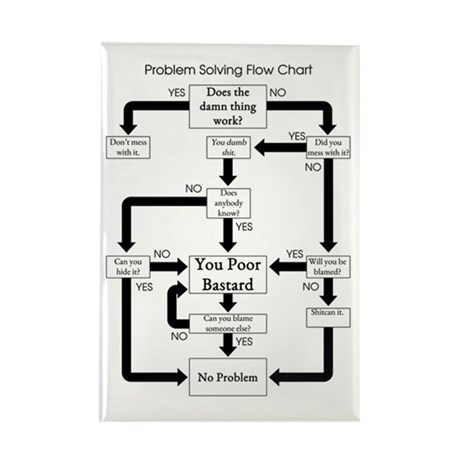
\includegraphics[width=\textwidth]{decision_tree}
\caption*{\tiny https://thenexttobestblogever.wordpress.com/2009/11/07/problem-solving-flowchart-2/}
\end{figure}
 \end{columns}
}


\begin{frame}{Objectives}
\begin{columns}
\column{0.5\textwidth}
\begin{itemize}
\item Quick review of Lecture 16 on regression trees
\begin{itemize}
\item Terminology
\item ``$T_0$''
\end{itemize}
\item How to choose the right tree via cross validation
\item Classification trees
\begin{itemize}
\item Same as regression, just different loss functions
\end{itemize}
\end{itemize}


\column{0.5\textwidth}
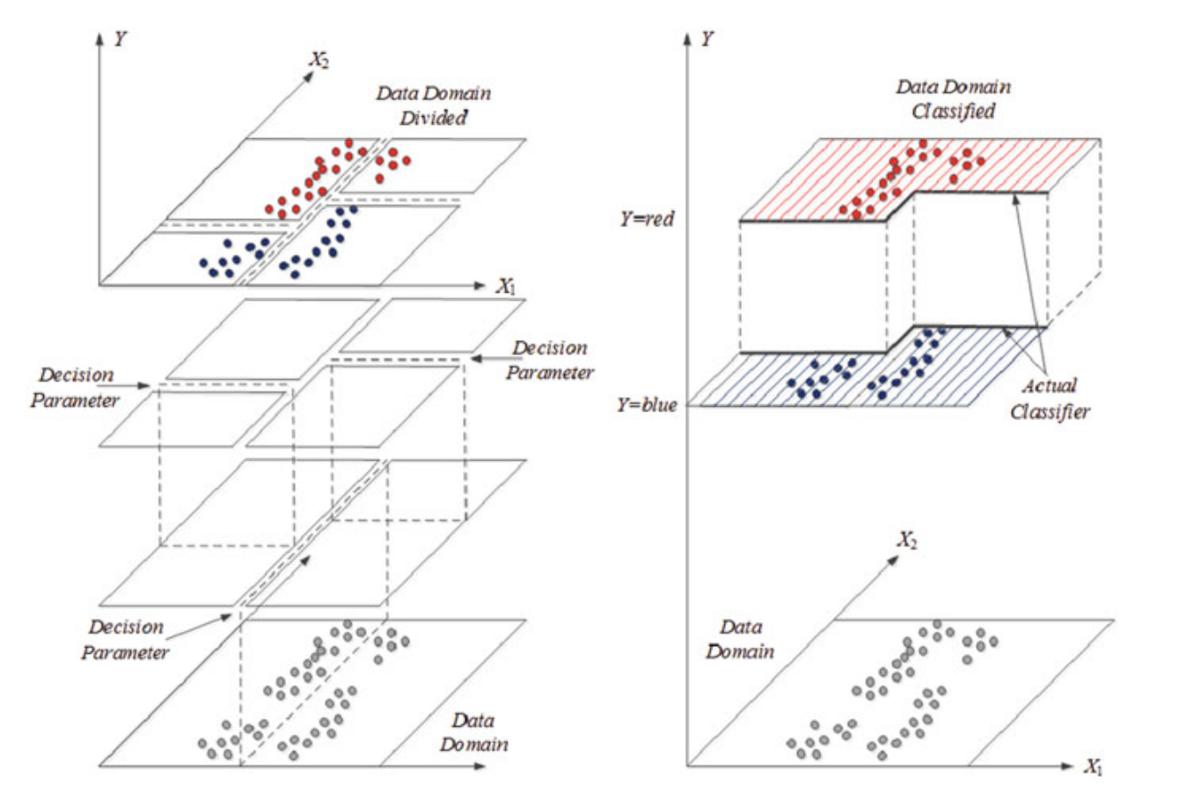
\includegraphics[width=\textwidth]{RTree_image}

{\tiny (medium.com)}
\end{columns}


\end{frame}



\begin{frame}{Terminology we'll cover...}
	\begin{itemize}
		\item Terminal node
		\item Internal node
		\item Branches
		\item Leaves
		\item Binary splits
		\item Recursive binary splitting $\leftrightarrow$ Top-down greedy 
		\item Cost complexity pruning
	\end{itemize}
\end{frame}

\begin{frame}{Basic idea for regression trees}

\begin{center}
All we are doing is ``splitting'' the observations into regions in the feature space, and averaging the response variable within each region.\\~\\
\pause
\end{center}

Doing predictions with the model just involves 
\begin{itemize}
\item locating a set of \textbf{features} in a region, 
\item then setting the response variable equal to\\ the \textbf{average} from the training \textbf{response}\\ variable in that region.  
\end{itemize}
\pause

\vspace{5mm}

Big decision in regression trees: \textit{What are the regions we should use?}
\end{frame}


\begin{frame}{Regression trees -- basic approach}

\begin{enumerate}
\item Divide the \textbf{feature} space into non-overlapping regions
\begin{itemize}
\item This distinguishes the method from KNN regression
\end{itemize}
\item Within each region, the prediction is just the average of the \textbf{response variable} from training data.
\begin{itemize}
\item This is similar to KNN regression
\end{itemize}
\end{enumerate}

\pause

Two Basic Questions:

\begin{enumerate}
\item Where should I put the internal nodes (i.e. the ``splits'')?
\item How many regions should there be?
\end{enumerate}

The answers are, as it turns out, really simple.  

\end{frame}



\begin{frame}{Where should the splits be?}

Then we partition any region by choosing $j$ and $s$ as follows:

\begin{align*}
\{j,s\} = \arg \min_{j\in J, s\in X_j} \sum_{i:x_i\in R_1(j,s)} (y_i-\hat{y}_{R_1})^2 + \sum_{i:x_i\in R_2(j,s)} (y_i-\hat{y}_{R_2})^2
\end{align*}
where $\hat{y}_{R_k}$ is the mean of all response variables in region k.  \\~\\

It would be tedious to identify $j$ and $s$ by hand, but it's actually very quick computationally.  

\vspace{5mm}
\textbf{Question:  How many $j$-$s$ pairs for $p$ features and $n$ observations?} \pause 
\begin{itemize}
	\item No more than $p(n-1)$, since we can only choose $(n-1)$ boundaries between observations.  
	\item There may be fewer, if separate observations share the same values for some of their features.
\end{itemize}
\end{frame}

\begin{frame}{Repeating the splits}

On each step, we're choosing the single best possible split from among the $R$ regions, resulting in $R+1$ regions to take to the next step. \\~\\

Repeat this process until you reach a stopping criterion -- typically a maximum number of observations in each region. (For example all regions have no more than 5 observations.) \\~\\ 

\textbf{Call the resulting tree $T_0$.} \\~\\

\textbf{We call this approach ``greedy''} because when we do the first partition we're not thinking ahead to future partitions to evaluate it.  


\end{frame}

\begin{frame}{One of these doesn't belong...}

\begin{figure}
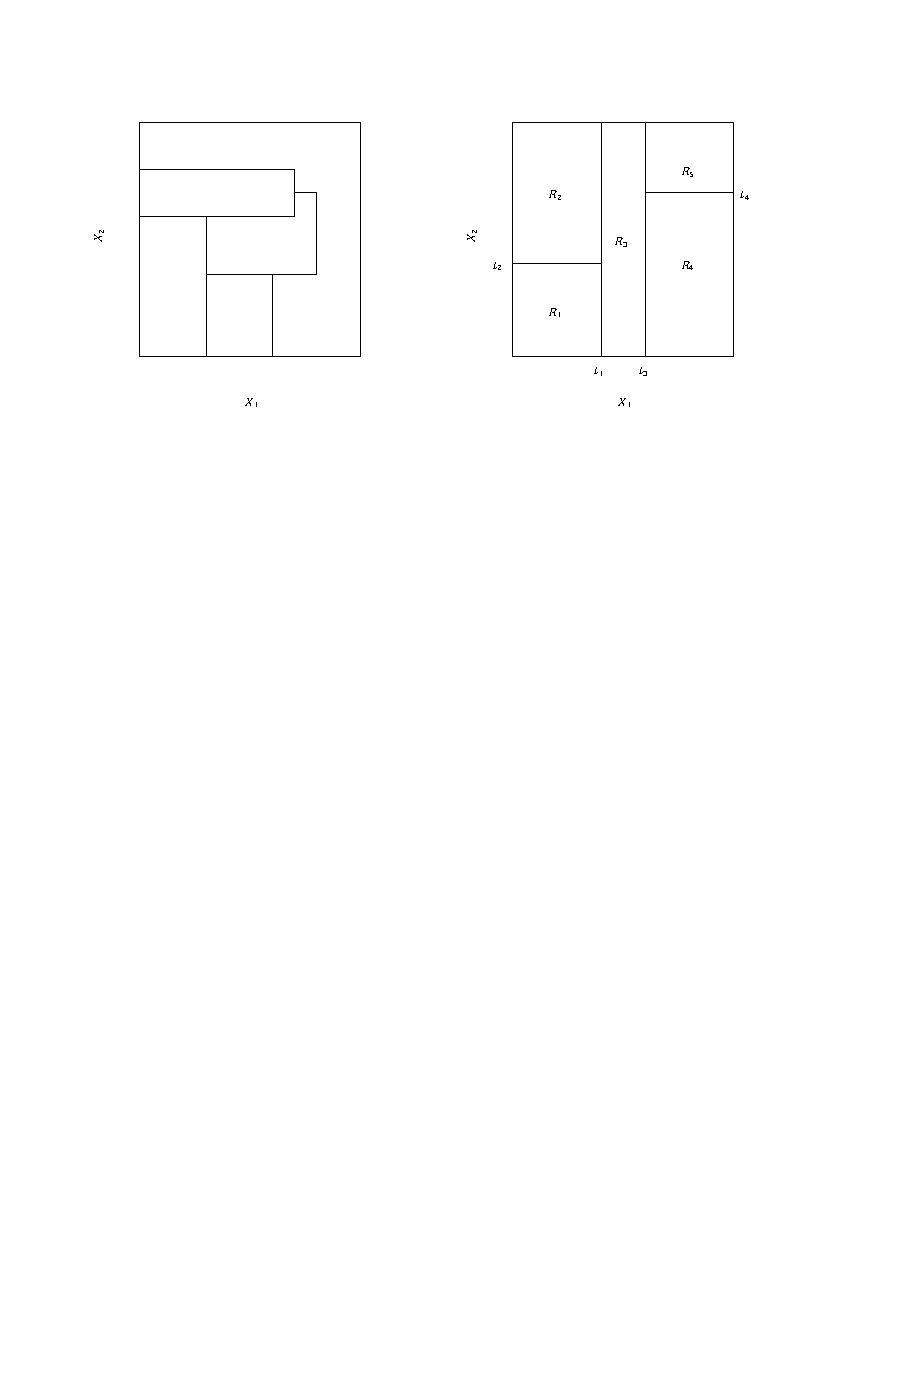
\includegraphics[width=0.8\textwidth]{partition_examples}
\caption*{}
\end{figure}

\vspace*{-10mm}

Q:  Which picture results from successively splitting the regions into values greater or less than feature values?\\~\\
\pause
A: The right one.  The left one is not possible with simple splitting.  
\end{frame}


\begin{frame}{A five region example... with two dimensional feature space}

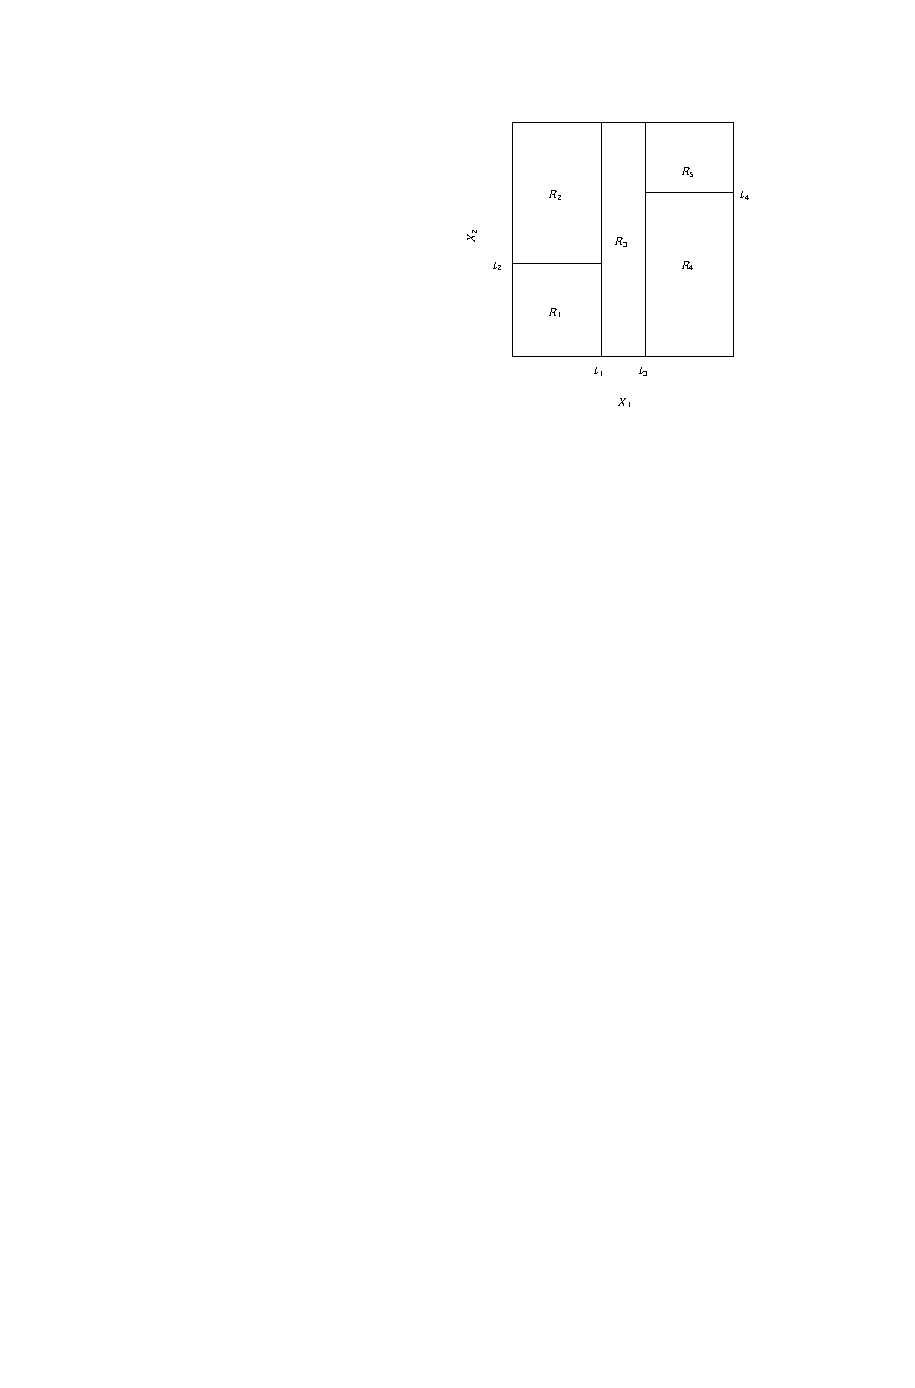
\includegraphics[width=0.3\textwidth]{five_region_ex_map}
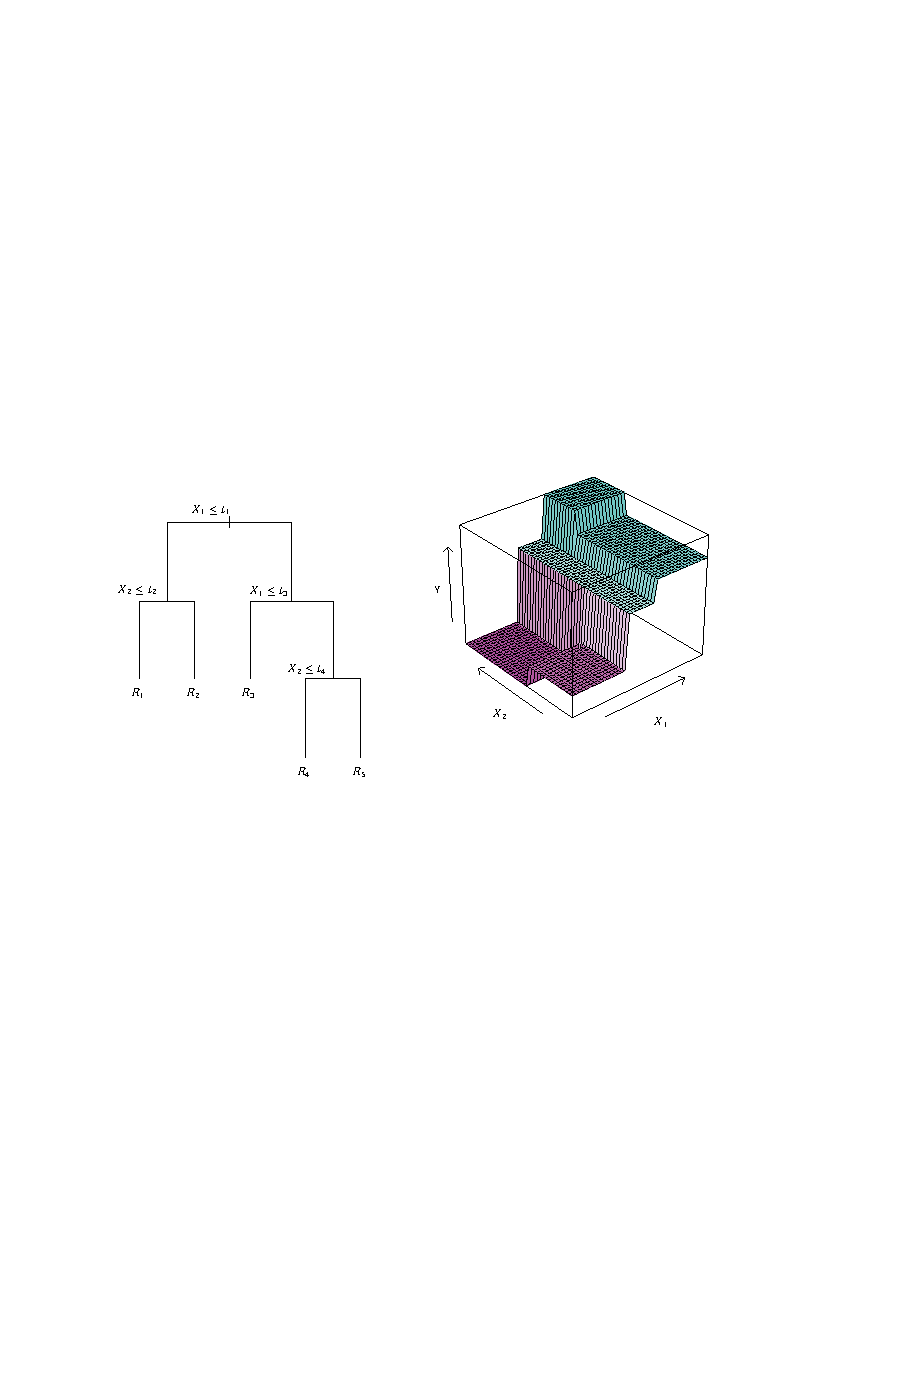
\includegraphics[width=0.7\textwidth]{five_region_ex}
\end{frame}

\begin{frame}{What do we call it?}

The process of splitting regions over and over is called...

\begin{center}
\textbf{``recursive binary splitting''}
\end{center}

You can also call it a \textbf{``top-down greedy'}' approach.  \\~\\

Because it's ``greedy'' we can't be sure that the splits we're getting are the best possible splits.  

\end{frame}

\begin{frame}{Why binary?}
In other words, why not multiway splits?\\~\\

\pause
In general multiway splits fragment the data too quickly, leaving insufficient data at the next level down\\~\\

Since we do the binary splitting recursively, we get the same flexibility as a multiway split, since a region can be split a second time later.
\end{frame}


\begin{frame}{Terminology so far...}
	\begin{itemize}
		\item Terminal node
		\item Internal node
		\item Branches
		\item Leaves
		\pause
		\item Binary splits
		\item Recursive binary splitting $\leftrightarrow$ Top-down greedy 
	\end{itemize}
\end{frame}

\begin{frame}{Example $T_0$}
\begin{columns}
\column{0.35\textwidth}
Remember, $T_0$ is the biggest tree we build.  We get there by recursively splitting until we meet a threshold (often a maximum number of observations per terminal node).
\column{0.65\textwidth}
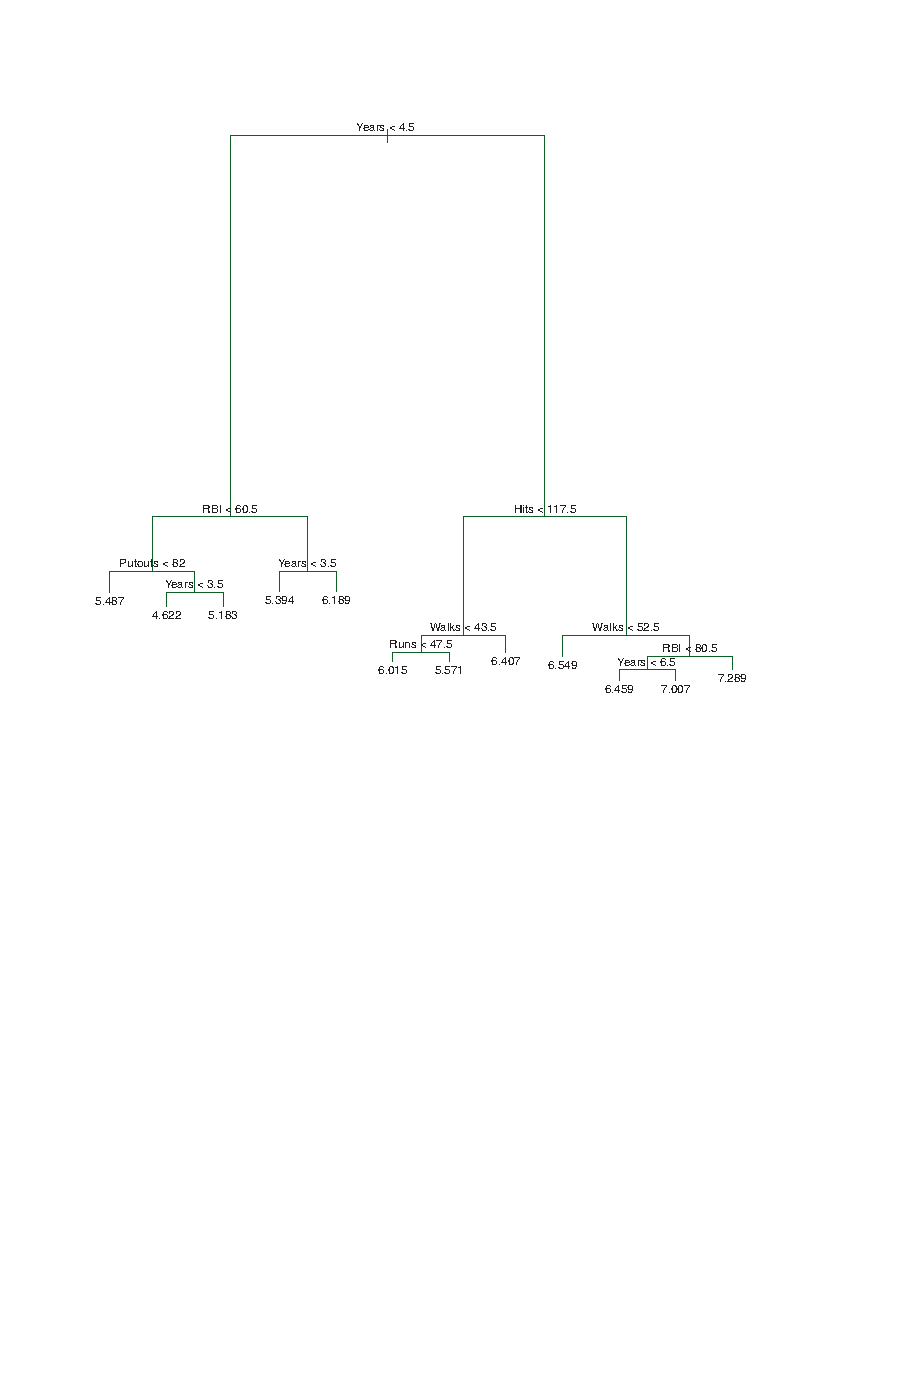
\includegraphics[height=0.9\textheight]{complex_tree}

\end{columns}

\end{frame}

\begin{frame}{When will we test?}

All the steps above involve model \textit{building}.  We have yet to evaluate different models against one another.  First let's build the candidate models, then we can evaluate.
\end{frame}

\begin{frame}{\textbf{Step 1: } ``cost complexity pruning''}

We'll test models that are \textbf{subtrees} of $T_0$. (trees that are the same as $T_0$ except they are missing some internal nodes and branches).\\~\\

We identify subtrees using \textbf{cost-complexity pruning} a.k.a. weakest link pruning:
\vspace{4mm}
\begin{itemize}
\item To get the first subtree, evaluate model performance for all subtrees with one leaf removed from $T_0$.  Choose the best one, call it $T_1$.  
\begin{itemize}
\item $R^2$ works for measuring performance
\item ...but not for categorical variables, stay tuned!
\end{itemize}
\vspace{4mm}
\item Then evaluate performance for all models with one leaf removed from $T_1$.  Choose the best, call it $T_2$.  And so on.  \\~\\
\end{itemize}

\pause

(Smart researchers have shown that this ``greedy'' approach is an optimal \textit{pruning} strategy.  But recursive binary splitting is not always optimal for growth.)

\end{frame}

\begin{frame}{\textbf{Step 2: } Tune up your $\alpha$}
Take your set of subtrees, $T_0$ through $T_{N-2}$.  Call $|T|$ the number of terminal nodes in the tree.\\~\\

For a given $\alpha$, \textit{one} of the $T_i$ will minimize :
\begin{align*}
\sum_{m=1}^{|T|} \sum_{x_i\in R_m} (y_i-\hat{y}_{R_m})^2+\alpha|T|
\end{align*}

\begin{itemize}
\item $\alpha=0$ will choose $T_0$, the biggest tree.
\item As $\alpha$ grows you'll choose successively smaller trees.  \\~\\
\end{itemize}

\end{frame}

\begin{frame}{Quick quiz}

For a given $\alpha$, \textit{one} of the $T_i$ will minimize :
\begin{align*}
\sum_{m=1}^{|T|} \sum_{x_i\in R_m} (y_i-\hat{y}_{R_m})^2+\alpha|T|
\end{align*}

Fill in the blank:  As $\alpha$ increases, bias goes \underline{\uncover<2->{\textbf{up}}} and variance goes \underline{\uncover<2->{\textbf{down}}}.  
%
\pause
%
Bigger $\alpha$ means fewer leaves, which means more bias but less variance.   \\~\\

Though it seems unnecessary to define $\alpha$ (why not just evaluate all subtrees?), we'll see it's useful for cross validation.  
\end{frame}

\begin{frame}{The (cross validation) process}

\begin{enumerate}
\item Split your data into $K$ folds.  
\vspace{3mm}
\item Repeat this process for each fold: Withhold the fold and for remaining training data:
\begin{enumerate}
\item[\textbf{a.}] Grow a large tree via recursive binary splitting.  ``Large'' means each leaf has some pre-specified maximum number of observations (e.g. 5)
\item[\textbf{b.}] Then ``prune'' the tree via cost complexity pruning to get a sequence of subtrees.  
\item[\textbf{c.}] Choose the tree in the sequence that minimizes $\sum_{m=1}^{|T|} \sum_{x_i\in R_m} (y_i-\hat{y}_{R_m})^2+\alpha|T|$ for each of a range of values of $\alpha$.
\item[\textbf{d.}] Record the test MSE (i.e. MSE on withheld fold) for each value of $\alpha$.
\vspace{3mm}
\end{enumerate}
\item Average the test MSE across all folds \textit{for each value of }$\alpha$, 
\vspace{3mm}
\item Choose the $\alpha$ that gives the lowest cross validated error, 
\vspace{3mm}
\item Build your final model with the chosen $\alpha$ with \textit{all the data.}
\end{enumerate}
\end{frame}

\begin{frame}{Why use $\alpha$?}

Why didn't we just evaluate cross validated error for each tree size?\\~\\

That is, is $\alpha$ just overly complicating things?\\~\\

\pause

Ans: Sometimes it might.  But it may be that across different folds we'd choose different subtrees.  $\alpha$ provides a better representation of the bias-variance tradeoff across folds.  \\~\\

But: out of convenience the book \textit{displays} results in terms of tree size rather than $\alpha$.  Argh!

\end{frame}


\begin{frame}{Terminology so far...}
	\begin{itemize}
		\item Terminal node
		\item Internal node
		\item Branches
		\item Leaves
		\item Binary splits
		\item Recursive binary splitting $\leftrightarrow$ Top-down greedy 
		\pause
		\item Cost complexity pruning
		\item Cross validation to choose best $\alpha$
	\end{itemize}
\end{frame}

%\begin{frame}{Results on Hitters data}
%\begin{figure}
%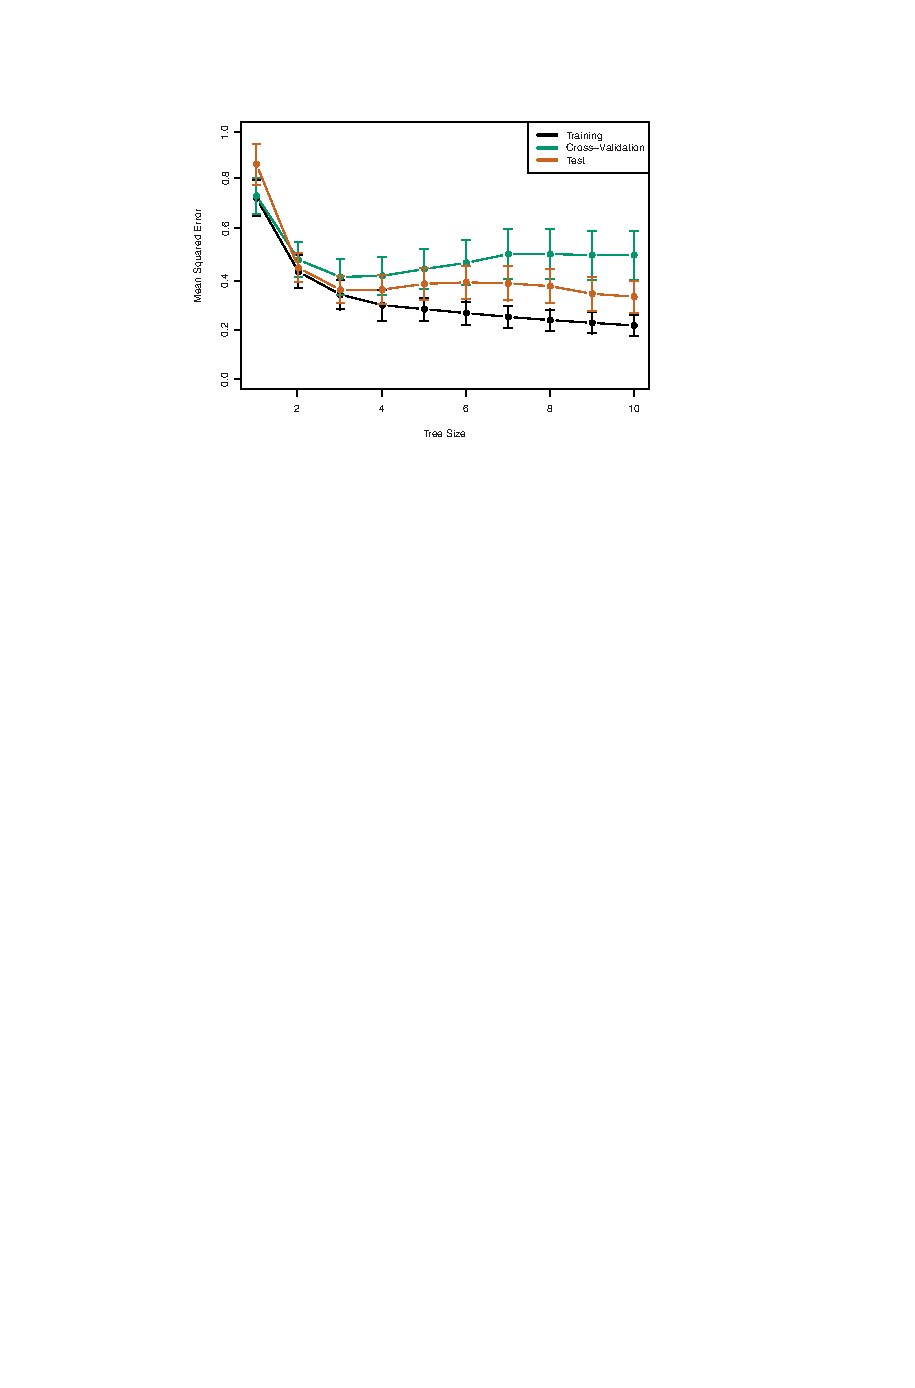
\includegraphics[width=0.8\textwidth]{MSE_vs_treesize}
%\caption*{``Training'' data are 132 of the 263 original observations.  Test are the reminaining.  CV is done just on the training data -- that is the training data are split into the K folds (6 in this case).  The test data are just used for additional evaluation.}
%\end{figure}
%\end{frame}

\begin{frame}{Questions}

Do regression trees utilize linear regression? \pause Nope.  \\~\\

What do you think their advantages are (vs LASSO or nonlinear models...)? \pause

\begin{itemize}
\item Easy to explain and non-experts can understand the results.
\item They're more like human decision-making.  Doctors like them.
\item They easily handle qualitative feature -- no need for dummies.
\end{itemize}

\pause How about some disadvantages? \pause

\begin{itemize}
\item As described, they don't usually provide the same predictive power that the other tools we've studied can.
\item They can be pretty sensitive to small changes in the data. 
\item Recursive binary splitting may generate a suboptimal tree (like forward / backward model selection).  Things later in the chapter address this.
\end{itemize}
\end{frame}

\end{document}
